\subsection{Generated Waste Data}
***description of waste calculator notebook for nuclear/wind/solar***

Coal power plants primarily produce solid wastes in the form of ash and slurries from the scrubbers.  Coal ash is produced from coal burning in approximately a 6:1 burned coal:coal ash ratio.  While the solid wastes are comprised of multiple elements, the waste is generally half coal ash, and half anhydrite ($CaSO_4$) - a product of chemical reactions in the scrubbers \cite{brown_solid_1996}.

\begin{figure}[h!]
\centering
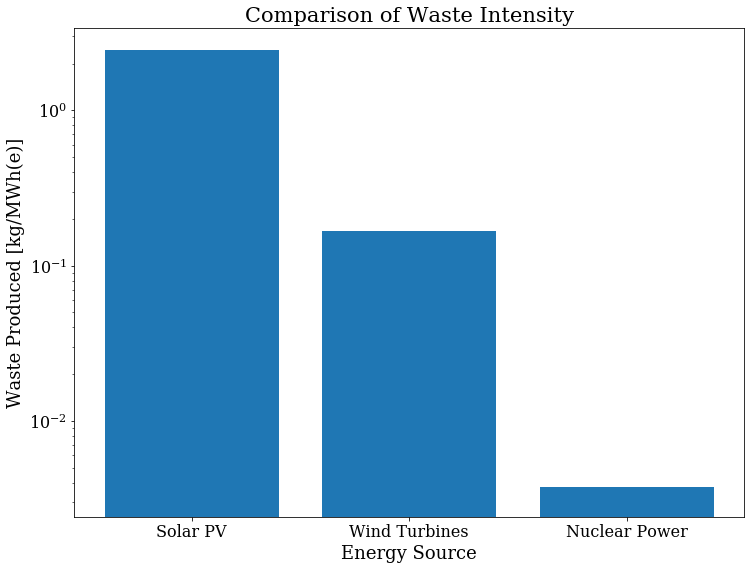
\includegraphics[width = 10cm]{img/mass-waste-intensity.png}
\caption{Solid Waste in $\frac{kg}{MWh}$ by Energy Source}
\label{fig:mass-waste}
\end{figure}
